\section{General GPU Architecture}
\label{sec:gpu}

The \textbf{General-purpose computation on graphics processing units (GPGPU)} is a microprocesser that performs computation traditionally handled by the CPU.
In our project we only work with CUDA-enabled devices, but we assume that the features of CUDA-enabled devices are equivalent to thoese of GPGPUs for the ease of notation.
The GPGPU consists of a large amount of simple and economical processing units that individually are weaker than the CPU, but combined possess upto several magnitudes of larger throughput.
The GPGPU is attached to the CPU, such that the CPU utilizes the GPGPU, to accelerate computation that the GPGPU is more suitable at handling, e.g. processes that are parallel.

\begin{figure}[htb]
  \centering
  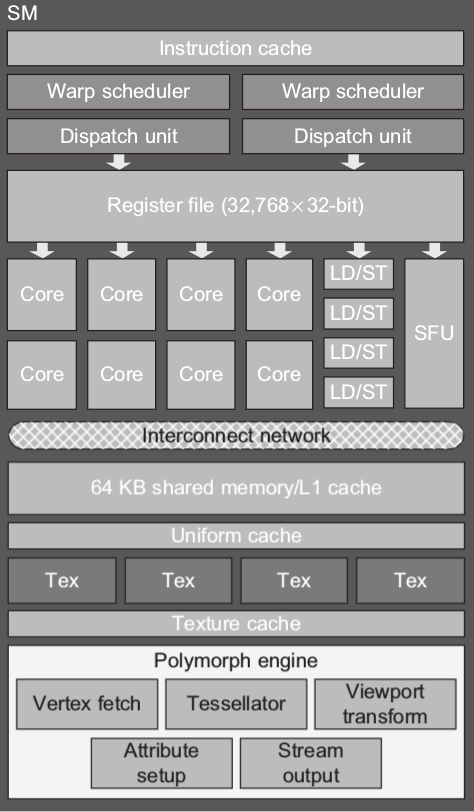
\includegraphics[width=.5\textwidth]{graphics/images/cropped-cuda-sm.png}
  \caption{Example of a Streaming Multiprocessor for reference~\cite{farber2011cuda}}
  \label{fig:sm example}
\end{figure}

The GPGPU's architecture is based on a parallel scheme, which has promoted an architecture of independance among processing cores on the GPGPU.
The basic building block of this architecture is the streaming multiprocessor (SM) shown in \cref{fig:sm example}, which is independently responsible for its own resources, cores, and memory.
By making each SM independent, memory access and computation are performed faster as the memory is placed physically closer to the cores.
The cores on each SM are Single Instruction, Multiple Data (SIMD) ALUs.
As the cores are constrained to run the same piece of code, though with different data, the software paradigm of ``kernels'' has developed.
A kernel is a describtion of a set of instruction that all cores across all SMs performs independantly of one another.

The work given to the GPU is distributed to the SMs by the Giga-Thread global scheduler.
The Giga-thread scheduler holds metainformation on the SMs, which allows it to optimize workloads across the GPGPU's independent processors.
The scheduling of work on a GPGPU is computed through ``blocks'', containing ``threads'' and organized in ``grids''.
The thread is an independant sequence of work, where the sequence is defined by instructions of the kernel.
A kernel can use its ID, compared to it's number in a set of threads, which it uses to coordinate its own work.
To organize threads and utilize the ability to communicate between threads on an SMs where memory access is fast, the concept of blocks has emerged.
A block containts a set amount of threads, has a set amount of L1 cache on the SM reserved and is able to synchronize between threads at any point in the kernel.
It further ensures that every thread is runned before terminating the block.
The grid is a set of blocks
The maximal number of threads a block can support is limited by hardware with 512 threads per block for older GPGPUs and 1024 for newer ones.

As overhead is incurred using  through A block is an extension of the thread that allows the thre a collection of threads being runned on the same SM, further the block has a set amount of memory allocated at the
theWhen a kernel is called from the host, the CPU, a Threads are the working unit of CUDA-enabled devicesThreads actually perform computations.
They are organised into blocks and grids.
These are described further in \cref{chap:software}.

The SMs receive instructions in a cache and warp schedulers distribute the work to the cores, so the instructions can be executed.
Each thread has access to its own registers, which is called its local memory.
Each SM has shared memory for high-speed data sharing between threads in a block.
The GPU as a whole has memory called global memory, which is accessible by all the GPU's SMs.

Furthermore, an SM has load/store (LD/ST) units and Special Function Units (SFU).
LD/STs calculate source and destination addresses and loads/store data as needed.
SFUs execute special functions, e.g. sin, sqrt, etc.
Each SFU executes one instruction per thread per clock.
SFUs can perform an operation while it is communicating with another thread.
Compared to the SIMD cores, the SFUs are designed specifically to perform their designated functions, and the SIMD cores are general purpose cores.

% good warp answers:  http://stackoverflow.com/questions/11816786/why-bother-to-know-about-cuda-warps
%                     http://stackoverflow.com/questions/10460742/how-do-cuda-blocks-warps-threads-map-onto-cuda-cores
A warp is a block of 32 SIMD threads, and they are the basic unit for scheduling work in the SMs.
To maximize the utilisation of the GPU the developer must make sure that these warp sizes are considered when executing code.
If one does not consider the warp size and randomly schedules tasks, then the programs might have many idle threads that do nothing.
If this is the case, then the GPU is not utilised to its optimal capacity~\cite{fermi2009nvidia}.

\subsection{Hardware Specific Numbers}
\label{sec:hardware specific numbers}

Throughout this report, we will be using the Tesla K40 GPU~\cite{teslak402013nvidia}.
For future reference \cref{tab:tesla k40 specs} presents the specifications for our GPU device.
In \cref{ap:tesla k40 specifications} we walk through how we found the specifications for our device.
\todo{is L1 cache used for shared memory?}

\begin{table}[htb]
  \centering
  \begin{tabular}{l r}
    \toprule
    item                        & limit \\
    \midrule
    warp size                   & \SI{32}{} \\
    max threads / block         & \SI{1024}{} \\
    total cores                 & \SI{2880}{} \\
    registers / block           & \SI{65536}{} \\
    constant memory             & \SI{65536}{B} \\
    L1 cache / block            & \SI{49152}{B}  \\
    L2 cache / core             & \SI{1572864}{B}  \\
    global memory               & \SI{12079136768}{B} \\
    \bottomrule
  \end{tabular}
  \caption{Tesla K40 GPU's specifications}
  \label{tab:tesla k40 specs}
\end{table}

Furthermore, the maximum dimension of grids and blocks are presented in \cref{tab:tesla k40 grid and block}.

\begin{table}[htb]
  \centering
  \begin{tabular}{r r r r}
    \toprule
    item & x & y & z \\
    \midrule
    block size & \SI{1024}{} & \SI{1024}{} & \SI{64}{} \\
    grid size  & \SI{2147483647}{} & \SI{65535}{} & \SI{65535}{} \\
    \bottomrule
  \end{tabular}
  \caption{Tesla K40 GPU's block and grid sizes}
  \label{tab:tesla k40 grid and block}
\end{table}
